\chapter{Puesta en marcha de benchmarks en los nodos del clúster Kabré}
Como parte del adecuado diagnóstico del clúster Kabré, se ponen en marcha benchmarks para determinar si el rendimiento es el adecuado para las distintas tareas que cada usuario desea efectuar en el equipo, así como es importante para saber si el equipo está funcionando adecuadamente y con el rendimiento esperado. De esta manera se vuelve vital ejecutar este tipo de pruebas. 

\section{High Performance Linpack Benchmark (HPL)}
HPL es un software el cual resuelve sistemas lineales densos aleatorios en sistemas computacionales de memoria distribuida con doble precisión \cite{linpack00}. El paquete ofrece programas de cronometrado y prueba para cuantificar la precisión de las soluciones obtenidas, junto con el tiempo transcurrido en la obtención de la solución. Tiene los siguientes requisitos mínimos \cite{linpack02}:

\begin{itemize}
\item Implementación de MPI 1.1
\item Implementación de BLAS o VSIPL
\end{itemize}

Se puede obtener la versión más reciente en el sitio \url{http://www.netlib.org/benchmark/hpl/}. Para descargarlo directamente en el clúster basta con hacer lo siguiente:

\begin{lstlisting}
wget http://www.netlib.org/benchmark/hpl/hpl-2.2.tar.gz # última versión al momento de realizar este manual
tar -xvzf hpl-2.2.tar.gz # para descomprimirlo
\end{lstlisting}

Una vez descargado y descomprimido, se procede a su compilación. Para ello hacemos lo siguiente \cite{linpack03}:

\section{(HPCG)}

\begin{lstlisting}
cd hpl-2.2
cp setup/Make.Linux_Intel64 .
nano Make.Linux_Intel64
\end{lstlisting}

El archivo que acabamos de copiar es un borrador de referencia para compilar los benchmarks para una arquitectura y sistema operativo específico, el cual el makefile utiliza como base. Antes de proceder a compilar, debemos modificarlo, de manera que se ajuste a las condiciones del equipo disponible. De primera entrada debemos modificar las siguientes líneas:

\begin{lstlisting}
# ----------------------------------------------------------------------
# - Platform identifier ------------------------------------------------
# ----------------------------------------------------------------------
#
ARCH         = Linux_Intel64
#
# ----------------------------------------------------------------------
# - HPL Directory Structure / HPL library ------------------------------
# ----------------------------------------------------------------------
#
TOPdir       = /root/hpl-2.2 # /opt/benchmarks/hpl-2.2 en caso de compilarlo en el directorio /opt
INCdir       = $(TOPdir)/include
BINdir       = $(TOPdir)/bin/$(ARCH)
LIBdir       = $(TOPdir)/lib/$(ARCH)
#
HPLlib       = $(LIBdir)/libhpl.a 
#
# ----------------------------------------------------------------------
# - Message Passing library (MPI) --------------------------------------
# ----------------------------------------------------------------------
# MPinc tells the  C  compiler where to find the Message Passing library
# header files,  MPlib  is defined  to be the name of  the library to be
# used. The variable MPdir is only used for defining MPinc and MPlib.
#
MPdir        = /opt/intel/impi/5.1.3.210 # path de la implementación de Intel de MPI
MPinc        = -I$(MPdir)/include64
MPlib        = $(MPdir)/lib64/libmpi.a

\end{lstlisting}

El resto de líneas pueden dejarse como están para empezar. Ya más adelante se podrá realizar un ajuste más fino de la mano con la documentación del benchmark y las necesidades que se tengan en el momento. Finalmente, compilamos el benchmark \cite{linpack01}:

\begin{lstlisting}
make
\end{lstlisting}

Este proceso de compilación generará un directorio bin/Linux\_Intel64 el cual contiene dos archivos: HPL.dat y xhpl. El HPL.dat contiene parámetros que se pueden modificar para ajustar las condiciones de las pruebas que se desea realizar. El archivo TUNING ofrece una guía de referencia para poder ajustar el archivo HPL.dat. El archivo xhpl es un ejecutable el cual toma lo establecido en HPL.dat y lo ejecuta. Para ejecutarlo basta con hacer lo siguiente:

\begin{lstlisting}
mpirun ./xhpl
\end{lstlisting}

Es posible proporcionar una lista de hosts para la ejecución del benchmark.

\begin{lstlisting}
mpirun -hostfile "nombre_del_archivo_o_env_var" ./xhpl
\end{lstlisting}

\subsection{Ajuste de parámetros del HPL.dat}
Como se indicó previamente, este archivo permite ajustar los parámetros de las pruebas de benchmarking. De acuerdo con la documentación disponible, se puede realizar incluso ajustes en el método de resolución de los sistemas \cite{linpack01}.

\begin{lstlisting}
HPLinpack benchmark input file
Innovative Computing Laboratory, University of Tennessee
HPL.out      output file name (if any)
6            device out (6=stdout,7=stderr,file)
4            # of problems sizes (N)
29 30 34 35  Ns
4            # of NBs
1 2 3 4      NBs
0            PMAP process mapping (0=Row-,1=Column-major)
3            # of process grids (P x Q)
2 1 4        Ps
2 4 1        Qs
16.0         threshold
3            # of panel fact
0 1 2        PFACTs (0=left, 1=Crout, 2=Right)
2            # of recursive stopping criterium
2 4          NBMINs (>= 1)
1            # of panels in recursion
2            NDIVs
3            # of recursive panel fact.
0 1 2        RFACTs (0=left, 1=Crout, 2=Right)
1            # of broadcast
0            BCASTs (0=1rg,1=1rM,2=2rg,3=2rM,4=Lng,5=LnM)
1            # of lookahead depth
0            DEPTHs (>=0)
2            SWAP (0=bin-exch,1=long,2=mix)
64           swapping threshold
0            L1 in (0=transposed,1=no-transposed) form
0            U  in (0=transposed,1=no-transposed) form
1            Equilibration (0=no,1=yes)
8            memory alignment in double (> 0)
\end{lstlisting}

\section{Graph500}



\section{Intel Math Kernel Library Benchmarks (MKL)}
El software para benchmarks provisto por Intel incluye LINPACK, HPCG y MP\_LINPACK, todos estos dentro del paquete Intel Math Kernel Library Benchmarks (MKL). Para proceder a la descarga del mismo, se debe ingresar al sitio \url{https://software.intel.com/en-us/articles/intel-mkl-benchmarks-suite} y proceder a descargar el paquete para Linux, tal y como se muestra en la figura \ref{fig:benchmark:00}

\begin{figure}[H]
\centering
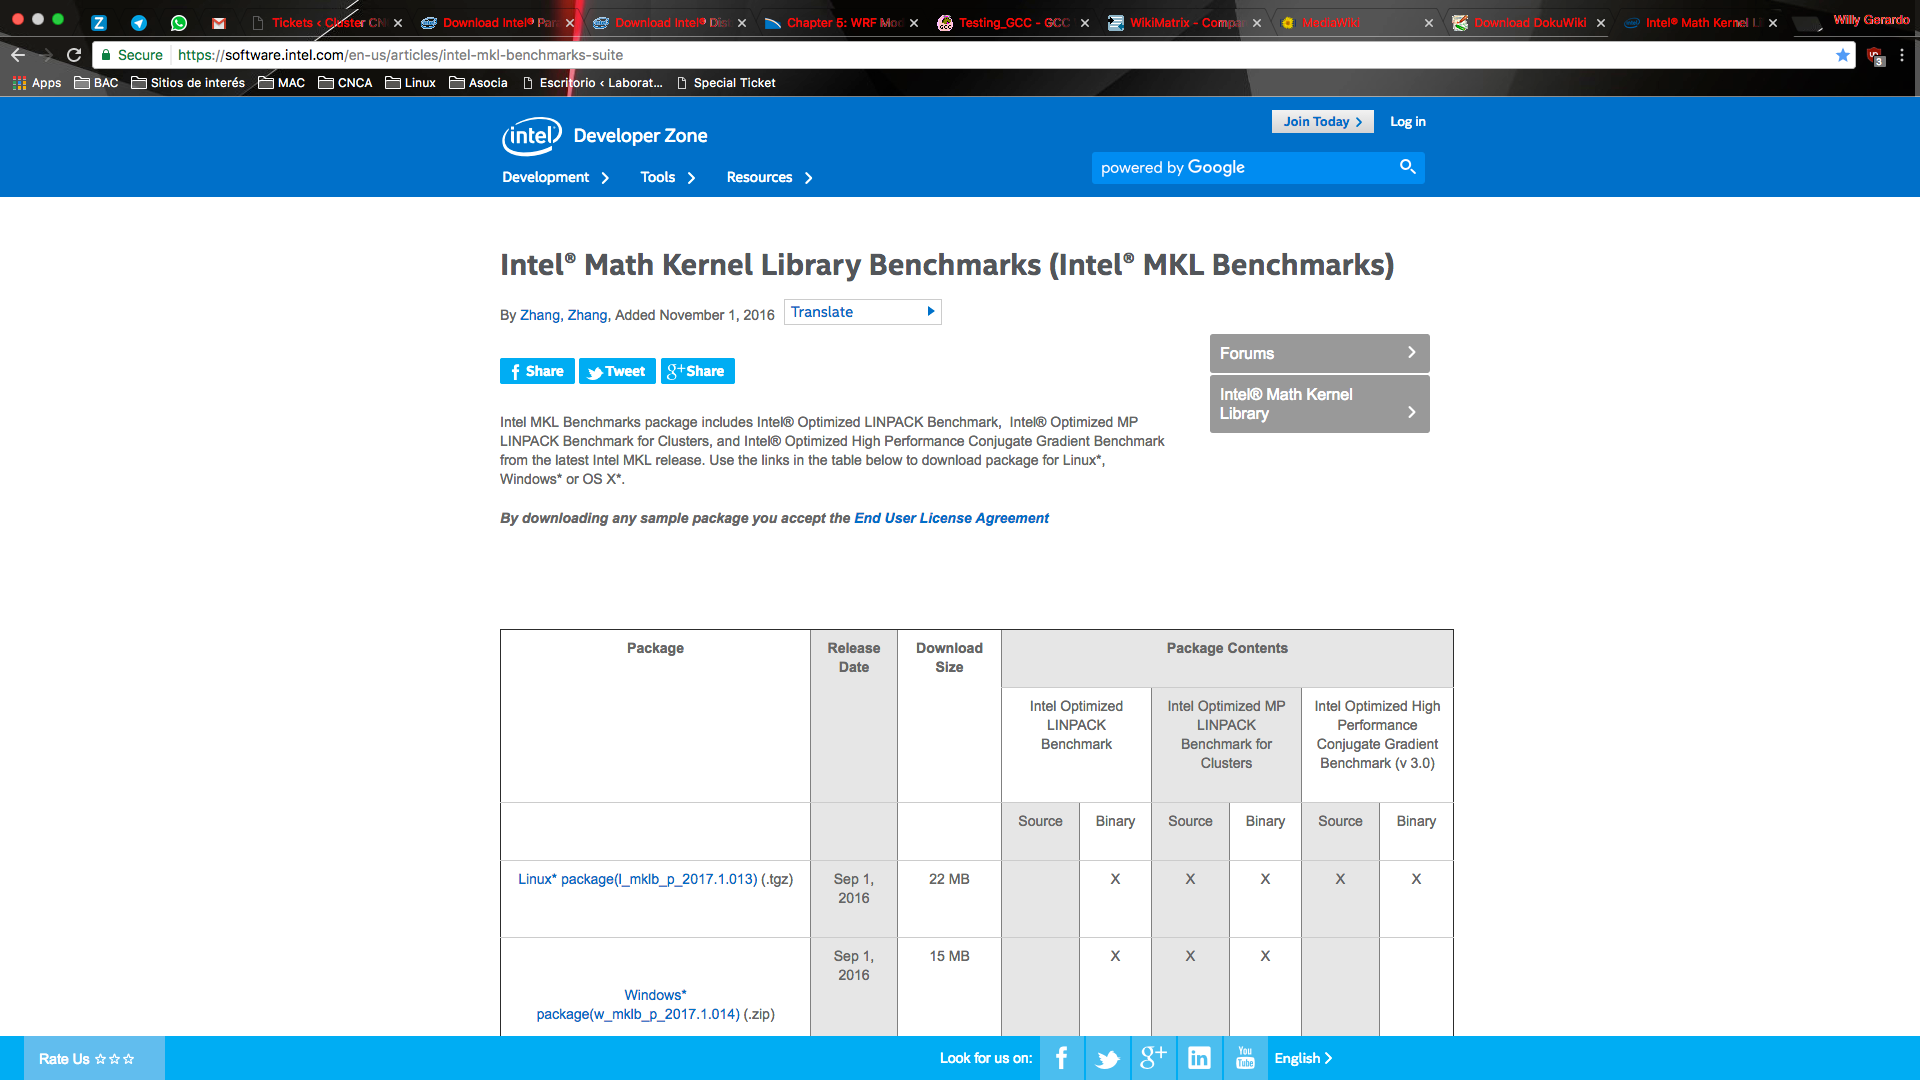
\includegraphics[width=0.6\textwidth]{mkl00.png}
\caption{Página de descarga de Intel MKL Benchmarks.}
\label{fig:benchmark:00}
\end{figure}


\clearpage